\renewcommand*{\arraystretch}{1.1}

\noindent\begin{tabularx}{17cm}{|p{1.95cm}|X|}
	\hline
	workload    & BI \\ \hline
%
	query       & 24 \\ \hline
%
	title       & Messages by Topic and Continent \\ \hline
	\multicolumn{2}{|c|}{ 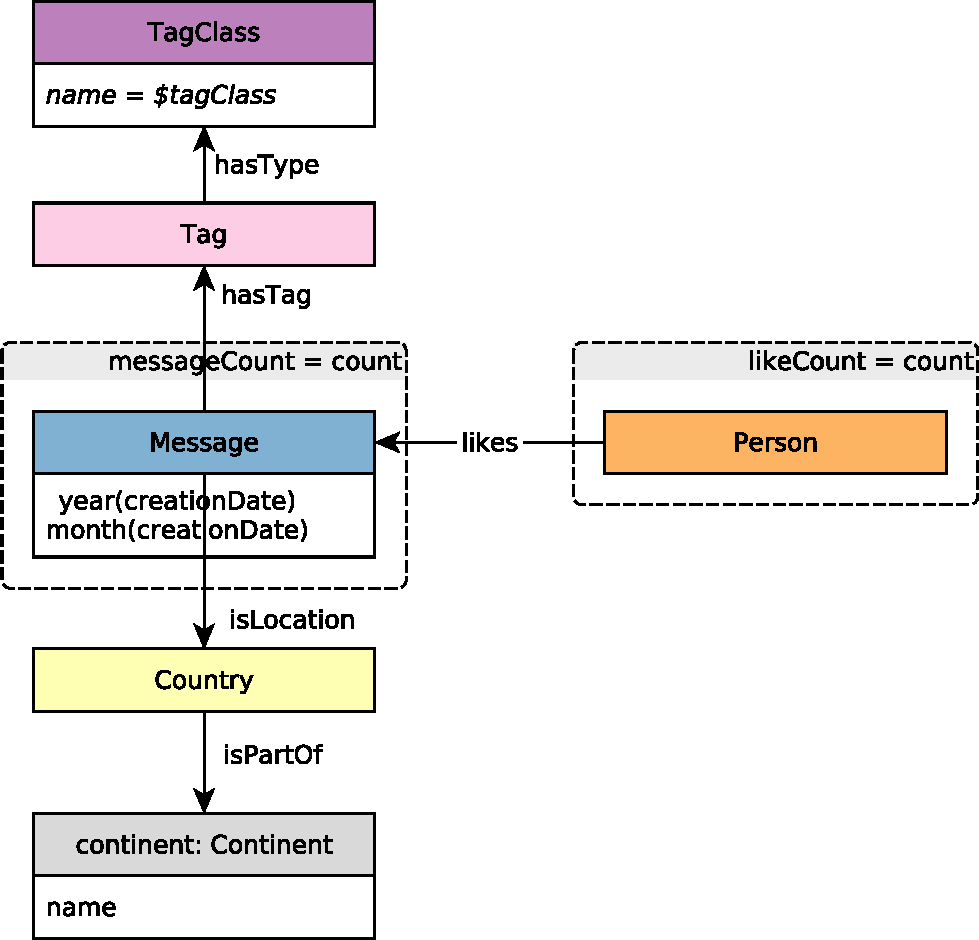
\includegraphics[scale=\patternscale,margin=0cm .2cm]{patterns/bi24}} \\ \hline
	description & Find all Messages tagged with a Tag from the given TagClass
(non-transitive).

Count all messages and their likes grouped by continent, year, and
month. (TODO - do we group the Messages or the Persons who liked the
Messages by continent? I think the former one - szarnyasg)
 \\ \hline
	
%
	group by       &
	\multicolumn{1}{>{\raggedright}X|}{
		\varname{year}, 
		\varname{month}, 
		\varname{continent.name}
		} \\ \hline
	
%
	parameters  &
	\vspace{1.1ex}{\begin{tabularx}{14.38cm}{|c|M|m{2cm}|Y} \hline
	\cellcolor{black!70} \color{white} $\mathsf{1}$ & \varname{tagClass} & \cellcolor{gray!20} \vartype{String} &  \\
	\end{tabularx}} \\ \hline
%
	result      &
	\vspace{1.1ex}{\begin{tabularx}{14.38cm}{|c|M|m{2cm}|Y} \hline
	\cellcolor{black!70} \color{white} $\mathsf{1}$ & \varname{messageCount} & \cellcolor{gray!20} \vartype{32-bit Integer} &  \\\hline
	\cellcolor{black!70} \color{white} $\mathsf{2}$ & \varname{likeCount} & \cellcolor{gray!20} \vartype{32-bit Integer} &  \\\hline
	\cellcolor{black!70} \color{white} $\mathsf{3}$ & \varname{year} & \cellcolor{gray!20} \vartype{32-bit Integer} & year of the Message's creationDate \\\hline
	\cellcolor{black!70} \color{white} $\mathsf{4}$ & \varname{month} & \cellcolor{gray!20} \vartype{32-bit Integer} & month of the Message's creationDate \\\hline
	\cellcolor{black!70} \color{white} $\mathsf{5}$ & \varname{continent.name} & \cellcolor{gray!20} \vartype{String} &  \\
	\end{tabularx}} \\ \hline
	%
	sort        &
	\vspace{1.1ex}{\begin{tabular}{|c|l|c|} \hline
	\cellcolor{black!70} \color{white} $\mathsf{1}$ & \varname{year} & \cellcolor{gray!20} $\asc$ \\\hline
	\cellcolor{black!70} \color{white} $\mathsf{2}$ & \varname{month} & \cellcolor{gray!20} $\asc$ \\\hline
	\cellcolor{black!70} \color{white} $\mathsf{3}$ & \varname{continent.name} & \cellcolor{gray!20} $\desc$ \\
	\end{tabular}} \\ \hline
	%
	limit       & 100 \\ \hline
	%
	choke points &
	\multicolumn{1}{>{\raggedright}X|}{
		\chokepoint{1.6}, 
		\chokepoint{2.1}, 
		\chokepoint{2.3}, 
		\chokepoint{2.4}, 
		\chokepoint{3.2}, 
		\chokepoint{4.3}
		}\\ \hline
\end{tabularx}
\clearpage